\documentclass{beamer}
\usepackage{listings}
\usepackage{graphics}
\usepackage{tabularx}
\graphicspath{{./}}
\usepackage[romanian]{babel}
\usepackage[utf8]{inputenc}
\usepackage{lmodern}
\usetheme{Warsaw}

\title[Testarea modelelor Acas XU folosind Nnenum și Alpha-Beta-CROWN]
{Testarea modelelor Acas XU folosind Nnenum și Alpha-Beta-CROWN}

\author[Vicol Mihai, Oșan Mihai, Bîzdoacă Mihai, Bogdan Topliceanu]
 {\textbf{Verificare Formală}}

\subsection{UNIVERSITATEA DE VEST DIN TIMIȘOARA, INFORMATICĂ}

\begin{document}
\begin{frame}
\titlepage
\end{frame}
\section{Introducere}
\subsection{UNIVERSITATEA DE VEST DIN TIMIȘOARA, INFORMATICĂ}
\begin{frame}
\begin{itemize}
	\item Verificarea rețelelor neuronale (Acas XU) cu ajutorul unor tool-uri specializate (Alpha-Beta-CROWN, Nnenum)
\end{itemize}

\end{frame}

\section{Dataset}
\subsection{UNIVERSITATEA DE VEST DIN TIMIȘOARA, INFORMATICĂ}
\begin{frame}
Acas XU
\begin{itemize}
  \item 	Detectarea aeronavelor în apropiere
  \item Estimarea stării aeronavelor
  \item Calcularea probabilității de coliziune
  \item Generarea instrucțiunilor de manevră

 \end{itemize}
\end{frame}
\begin{frame}
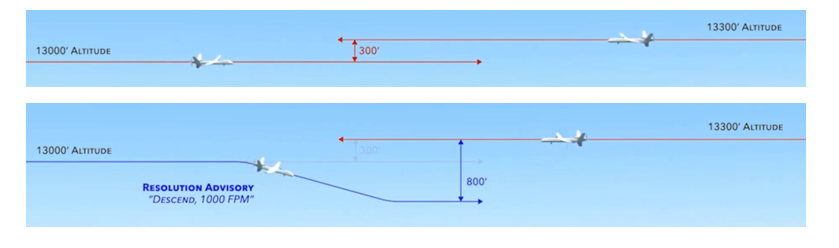
\includegraphics[scale=0.6]{acasxu.png}
\end{frame}

\section{Tool-uri}
\subsection{UNIVERSITATEA DE VEST DIN TIMIȘOARA, INFORMATICĂ}
\begin{frame}
Nnenum
\begin{itemize}
\item instrument pentru verificarea rețelelor neuronale care folosesc funcția de activare RELU
\item folosește diferite nivele de abstractizare pentru a îmbunătăți timpul de execuție
\item Instalare și rulare folosind imagini docker
\item penalizare pentru modelul 1\_9 proprietatea 7

 \end{itemize}
\end{frame}

\begin{frame}
Alpha-Beta-CROWN
\begin{itemize}
	\item verificator rețea neuronală bazat pe un framework de propagare liniară și branch and bound
	\item accelerare eficientă folosind GPU cu Pytorch si CUDA
    \item scalabil pentru rețele convoluționale mari
\end{itemize}
\end{frame}

\section{Rezultate}
\subsection{UNIVERSITATEA DE VEST DIN TIMIȘOARA, INFORMATICĂ}
\begin{frame}
Nnenum
\begin{tabularx}{1\textwidth}{ | >{\centering\arraybackslash}X | >{\centering\arraybackslash}X | X | X | X | X | X | }
  \hline
   Tool & Verified & Falsified & Fastest & Penalty & Score & Percent \\
\hline
   Nnenum & 139 & 47 & 0 & 0 & 1860 & 100 \\
\hline
   Rezultat Competitie & 139 & 47 & 0 & 0 & 1860 & 100 \\
\hline
\end{tabularx}
\end{frame}

\begin{frame}
\begin{center}
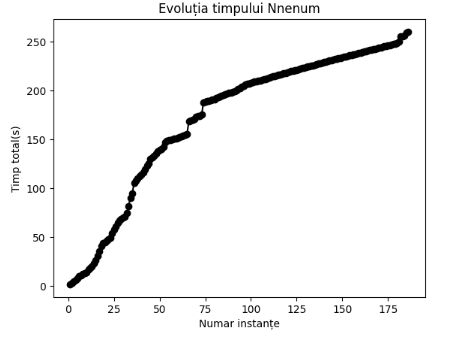
\includegraphics[scale=0.4]{timp_nn.png}
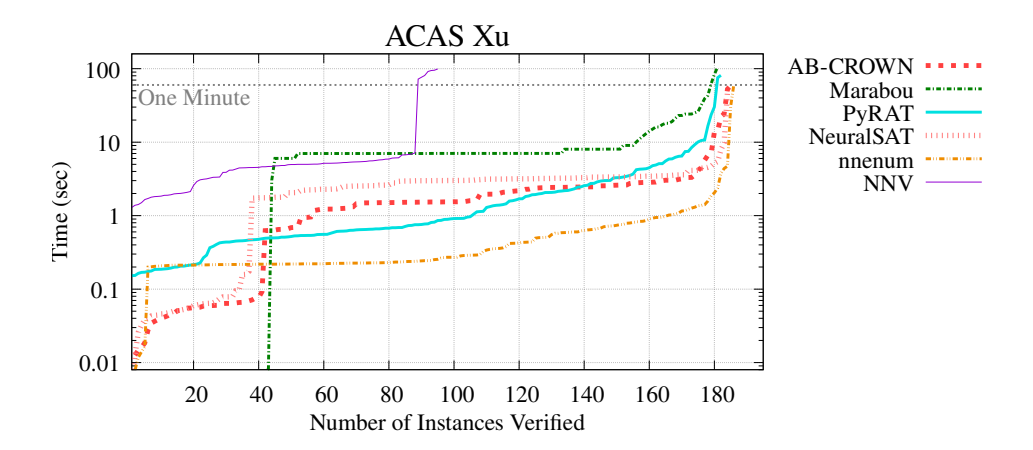
\includegraphics[scale=0.4]{vnncomp.png}
\end{center}
\end{frame}

\begin{frame}
Alpha-Beta-CROWN
\begin{tabularx}{1\textwidth}{ | >{\centering\arraybackslash}X | >{\centering\arraybackslash}X | X | X | X | X | X | }
  \hline
   Tool & Verified & Falsified & Fastest & Penalty & Score & Percent \\
\hline
   Alpha-Beta-Crown & 138 & 46 & 0 & 2 & 1540 & 74.19 \\
\hline
   Rezultat Competitie & 139 & 46 & 0 & 1 & 1700 & 91.4 \\
\hline
\end{tabularx}
\end{frame}

\begin{frame}
\begin{center}
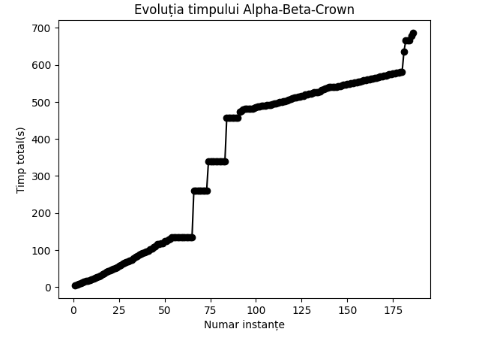
\includegraphics[scale=0.4]{timp_ab.png}
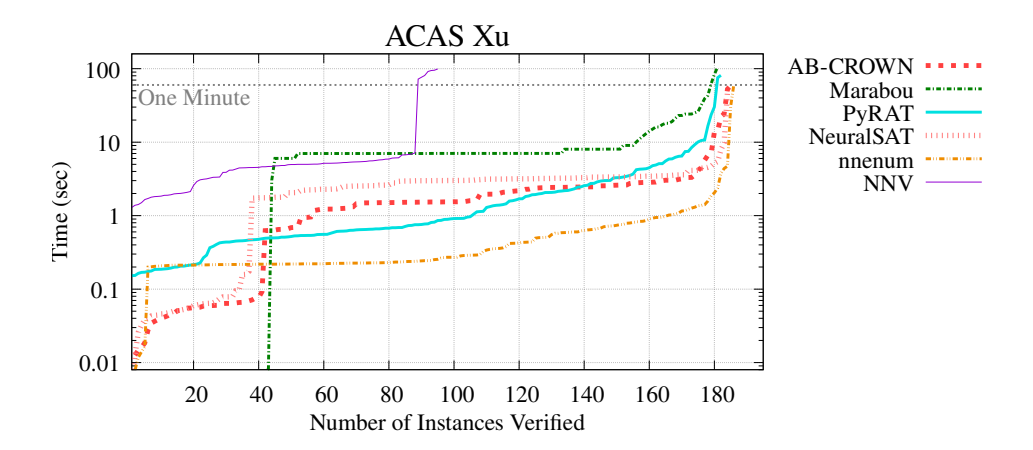
\includegraphics[scale=0.4]{vnncomp.png}
\end{center}
\end{frame}



\end{document}